\documentclass[aspectratio=169,11pt]{beamer}

\usetheme{Singapore}
\usepackage[utf8]{inputenc}
\usepackage{amsmath}
\usepackage{amsfonts}
\usepackage{amssymb}
\usepackage{graphicx}
\usepackage{hyperref}

% Setup the bibliography
\usepackage[style=authortitle,backend=bibtex]{biblatex}
\addbibresource{bibliography.bib}
\setbeamertemplate{bibliography item}[text]
\setbeamerfont{footnote}{size=\tiny}

% Allow footnotes with no number
\newcommand\blfootnote[1]{%
  \begingroup
  \renewcommand\thefootnote{}\footnote{#1}%
  \addtocounter{footnote}{-1}%
  \endgroup
}

% Allow section title slides
\AtBeginSection[]{
  \begin{frame}
  \vfill
  \centering
  \begin{beamercolorbox}[sep=8pt,center,shadow=true,rounded=true]{title}
    \usebeamerfont{title}\insertsectionhead\par%
  \end{beamercolorbox}
  \vfill
  \end{frame}
}

\author{Dr Stephen Pederson}
\title{Lecture 1: Introduction to the Transcriptome}
\subtitle{BIOINF3005/7160: Transcriptomics Applications}
%\setbeamercovered{transparent} 
\setbeamertemplate{navigation symbols}{} 
\logo{
	\includegraphics[scale=0.3]{figures/UoA_logo_col_vert.png} 
} 
\institute{Bioinformatics Hub, \\The University of Adelaide} 
\date{March 2nd, 2020} 
\subject{BIOINF3005/7160: Transcriptomics Applications} 


\begin{document}

\begin{frame}
\titlepage
\end{frame}

\begin{frame}
\footnotesize
\tableofcontents
\end{frame}

\section{University Statement}

\begin{frame}{Welcome to the University of Adelaide}

	\begin{itemize}
		\item The start of any academic year is an exciting time - but it can also be challenging for our students, for many reasons
		\item For some of our students, this year is especially challenging
		\item That's because many of our students who wanted to be here to study can't be here - because of COVID-19 and the travel restrictions to Australia
		\item This is not a situation that those students - or any of us in this room today - have any direct control over
		\item We may have some students watching this very lecture from overseas
	\end{itemize}
	
\end{frame}

\begin{frame}{Welcome to the University of Adelaide}

	\begin{itemize}
		\item Before the lecture begins, there are some points worth making so that everyone understands what the current situation is here at the University of Adelaide
		\item We have a diverse, inclusive, and welcoming community at our University, which is something we're very proud of
		\item In times of difficulty, that community is more important than ever.
		\item This is a time when our community comes together as a whole so we can care for and support each other together
		\item It's particularly important for those who may be going through a more difficult time than otherwise. 
		\item We must be respectful of other people - and that includes the many students who couldn't join us in the room today
	\end{itemize}

\end{frame}

\begin{frame}{COVID-19}

	\begin{itemize}
		\item The impact of COVID-19 is being felt right around the world. 
		\item The University's own response to COVID-19 is being shaped by the latest advice from the Government and from health authorities. 
		\item So far, there have only been a small number of COVID-19 cases in Australia ... only three in South Australia  ... and none at the University.	
		\item There is no evidence of transmission within the general community in Australia.
		\item Health authorities are advising we take the same basic precautions we would when it's cold or flu season – wash your hands, cover your mouth, dispose of tissues.
		\item This is good advice for any time you have a cough or a cold.	
 
	\end{itemize}

\end{frame}

\begin{frame}{COVID-19}

	\begin{itemize}
		\item There are resources available for students who need someone to talk to:
		
		\begin{itemize}
			\item Student Life, if you need some extra assistance or support
			\item Our Safer Campus Community website has a lot of resources to help us address harassment, including ways to report and get help
			\item Adelaide UniCare is our on-campus medical service, and you can make appointments online.
		\end{itemize}
		
		\item The University also has an online FAQ page about COVID-19 that's being constantly updated - there's a banner on our main webpage that links to the FAQ.
		\item The University has made it very clear that the safety and well-being of staff and students is paramount, and we will communicate with you clearly if anything changes.
		\item Welcome again, and good luck with your studies.
	\end{itemize}

\end{frame}


\section{Course Details}

\linespread{1.3}

\begin{frame}{Key Contacts}

	\begin{itemize}
		\item Prof David Adelson, \textit{Chair of Bioinformatics, Course Coordinator,} Room 261, The Braggs
		\item Dr Dan Kortschak, \textit{Program Coordinator, M Bioinformatics,} Room 260, The Braggs
		\item Dr Stephen Pederson, \textit{Coordinator, Bioinformatics Hub,} Room 420, Santos Petroleum Engineering Building
	\end{itemize}

\end{frame}

\begin{frame}{Course Timetable}

	\begin{itemize}
		\item Lectures:
		\begin{itemize}
			\item Monday 9:10am - 10:00am, Room B18, Ingkarni Wardli
\end{itemize}		 
		\item Practicals:
		\begin{itemize}
			\item Wednesday 9:10am - 11:00am, Room 111, Johnson Building
			\item Friday 9:10am - 11:00am, Room 111, Johnson Building
		\end{itemize}
	\end{itemize}

\end{frame}

\begin{frame}{Course Outline}

	\begin{itemize}
		\item Discussion of underlying biology
		\item Experimental approaches utilised in transcriptomic analysis
		\item Statistical and computational approaches utilised in transcriptomic analysis
		\item Practicals will be entirely computational
		\begin{itemize}
			\item Focussed on working in \texttt{R} with some \texttt{bash}
		\end{itemize}
	\end{itemize}

\end{frame}

\begin{frame}{Assessment}

	\begin{itemize}
		\item Continuous Assessment (\textit{i.e. no exam})
		\item 6 assignments (+ Major Project for BIOINF7160)
		\item Assessment is strongly focussed on practical material
		\item Attendance at practicals is not compulsory, but is \textbf{strongly advised}
	\end{itemize}

\end{frame}

\begin{frame}{Results from 2019 (BIOTECH7005)}

	\begin{center}
	\includegraphics[scale=0.5]{figures/biotech7005_2019pca.pdf} 	
	\end{center}

\end{frame}

\section{Why Transcriptomics?}

\linespread{1.05}

\begin{frame}{The Transcriptome}

	\begin{block}{Definition}
	The transcriptome can be defined as the complete set of (RNA) transcripts in a cell, or a population of cells, for a specific developmental stage or physiological condition\footfullcite{pmid19015660}
	\end{block}
	
	\begin{block}{Transcriptomics}
	Transcriptomics is simply the study of the transcriptome
	\end{block}
	

\end{frame}

\begin{frame}{The Transcriptome}

	The transcriptome can be summarised as the \textit{RNA content of a cell}.\\[3mm]
	
	\begin{itemize}
		\item Can include messenger RNA (\textit{mRNA}), non-coding RNA (\textit{ncRNA}), small RNA (\textit{miRNA, piRNA etc.})
		\item Can also include transfer RNA (\textit{tRNA}) and ribosomal RNA (\textit{rRNA})
		\item Nearly all RNA is single-stranded (\textit{ssRNA})
	\end{itemize}
	
	\vspace{3mm}
	
	We are always dealing with a \textbf{snapshot of a dynamic process} at the time we collected data

\end{frame}

\begin{frame}{Why Study The Transcriptome?}

	\begin{itemize}
		\item \textit{mRNA} is the intermediary step between the genome (DNA) and proteins
		\item small RNA and \textit{ncRNA} play significant roles in gene regulation
		\item Make inference about the \textbf{biological processes driving our observations}
		\begin{itemize}
			\item Targets for curing disease
			\item Biomarkers for tumour detection
			\item Understanding drought/salinity tolerance
		\end{itemize}

	\end{itemize}
	
\end{frame}

\begin{frame}{The Central Dogma of Molecular Biology}

	A common (but simplistic) version of the Central Dogma:
	
	\vspace{3mm}	
	
	\begin{center}
	\includegraphics[scale=1]{figures/Watson_Central_Dogma.jpg} 	
	\end{center}
	
	\vspace{3mm}	
	
	\begin{block}{}
	DNA makes RNA makes Protein.
	(Figure taken from \textit{The Molecular Biology of the Gene}\footfullcite{watson1965}, p298)
	\end{block}
	
	
\end{frame}

\begin{frame}{The Central Dogma of Molecular Biology}

	According to Crick\footfullcite{crick1956} 

	\begin{center}
	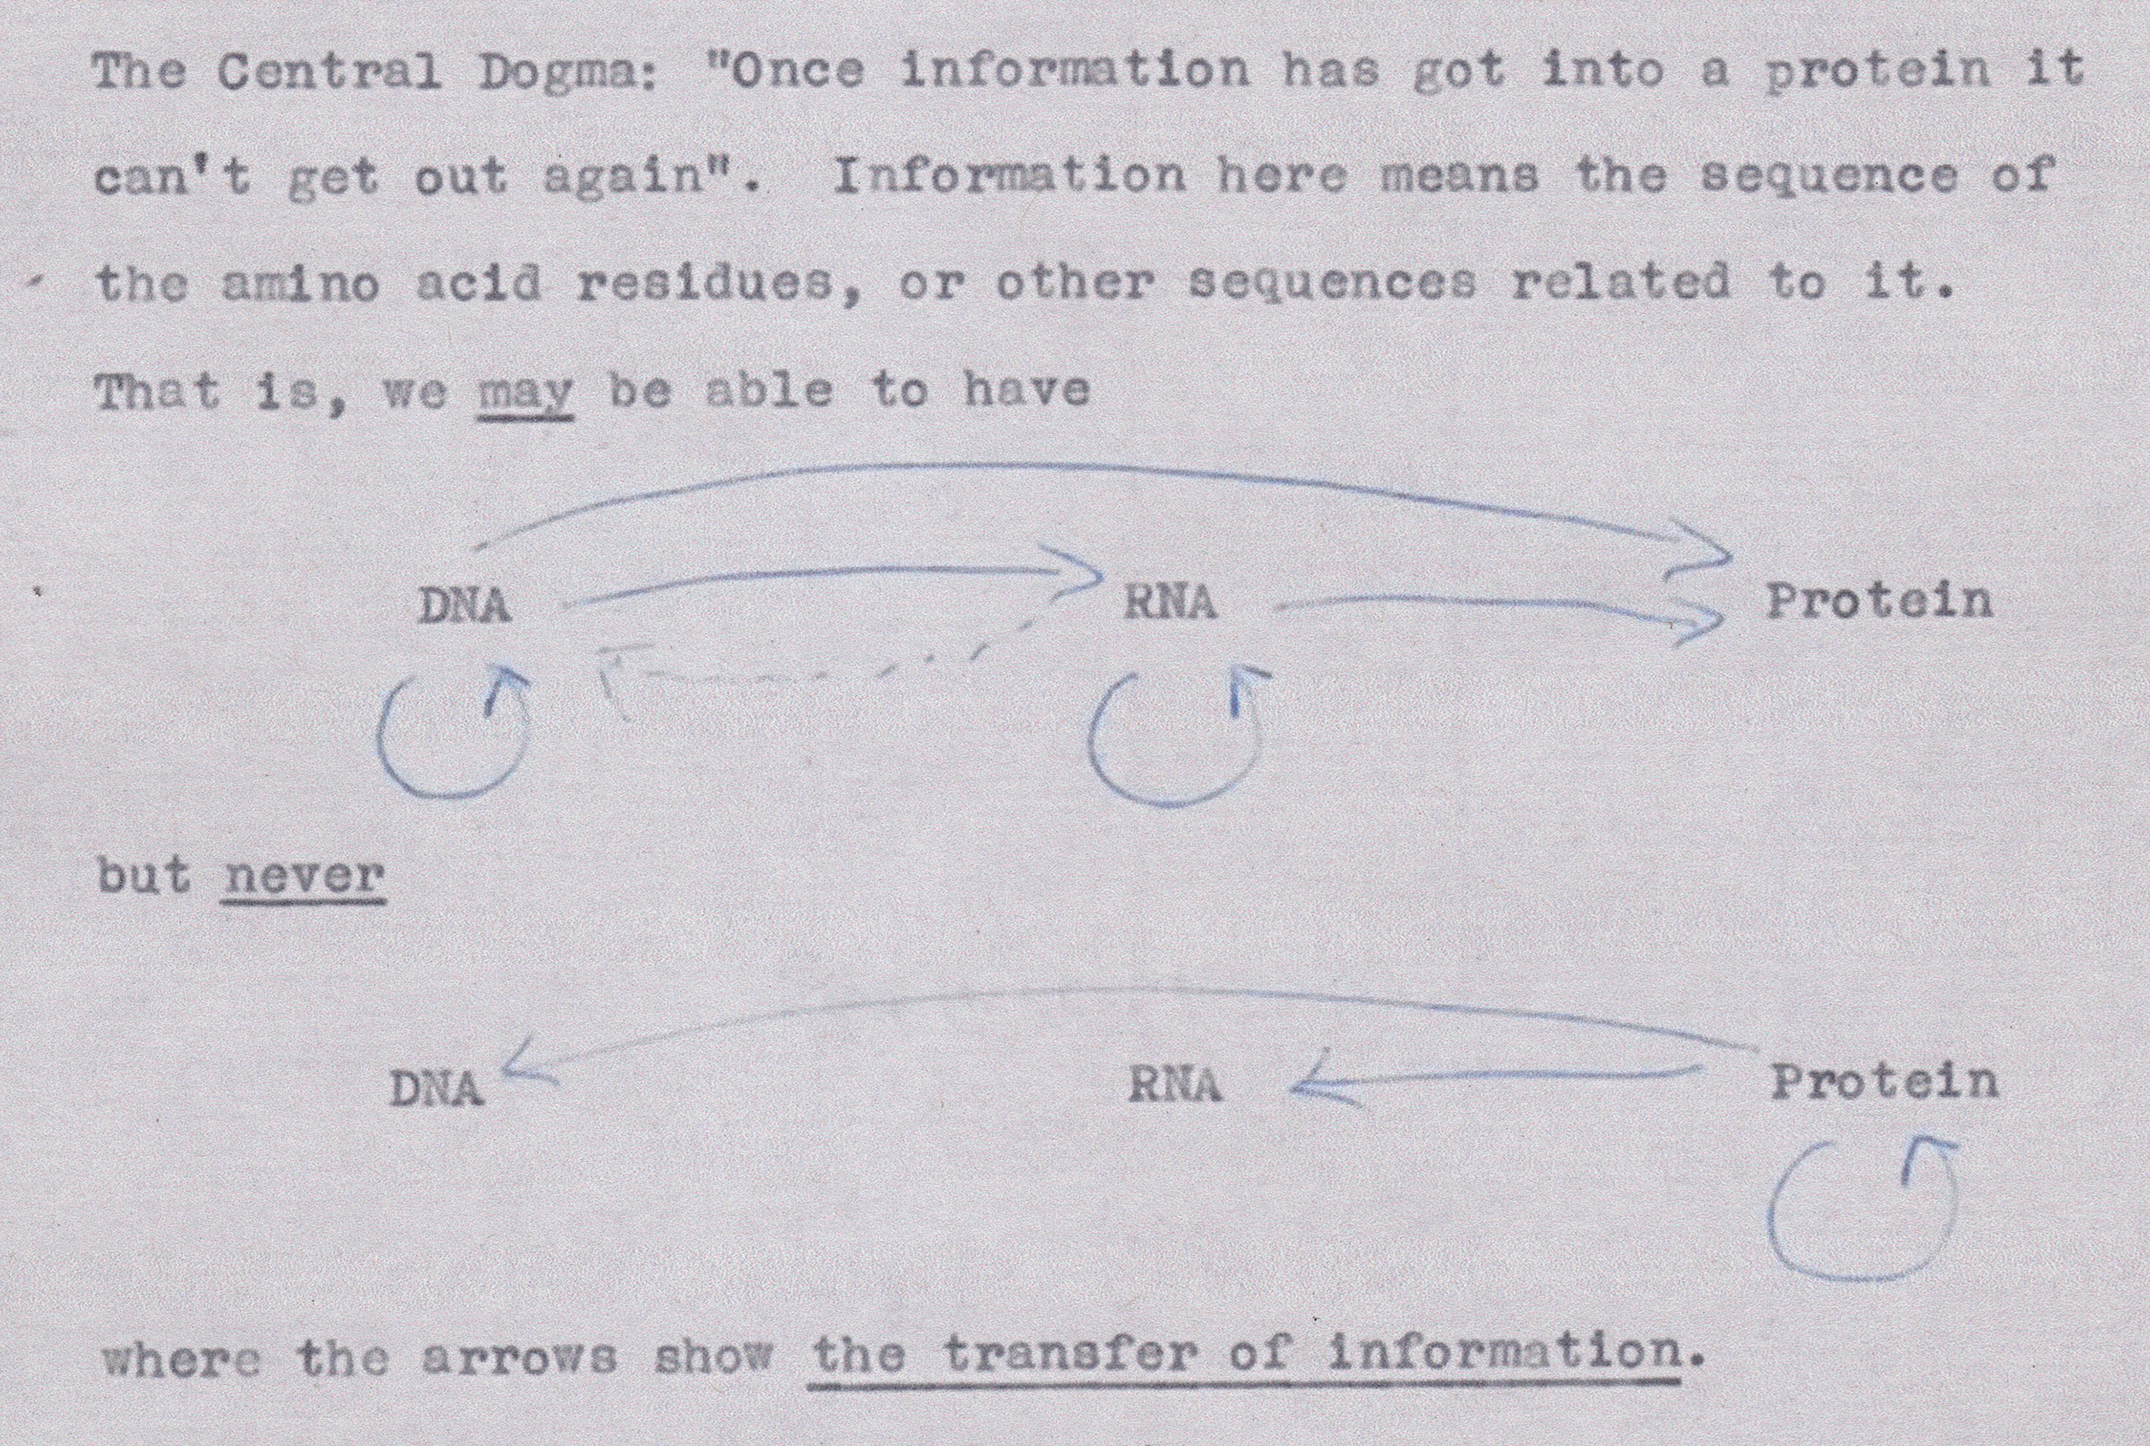
\includegraphics[scale=0.45]{figures/crick_dogma_note.png}
	\end{center}
	

\end{frame}

\begin{frame}{RNA Vs Protein}

A common assumption is: RNA abundance $\propto$ Protein abundance

	\begin{itemize}
		\item This can be true, but \textit{doesn't have to be true}
		\item Changes in gene expression indicate \textit{key biological responses} to a stimulus
		\item Transcriptomic analysis is often about a \textit{dynamic process}
		\item Often involves measuring and comparing RNA abundance (i.e. expression levels) in more than one condition
	\end{itemize}

\end{frame}


\section{Key Definitions}


\begin{frame}{What is a Gene?}

	\begin{block}{Definition}
		The gene is the basic physical unit of inheritance. 
		Genes are passed from parents to offspring and contain the information needed to specify traits. 
		Genes are arranged, one after another, on structures called chromosomes. 
		A chromosome contains a single, long DNA molecule, only a portion of which corresponds to a single gene. 
		Humans have approximately 20,000\footnote{This number is clearly not correct} genes arranged on their chromosomes.\footnote{https://www.genome.gov/genetics-glossary/Gene}
	\end{block}
	
\end{frame}


\begin{frame}{What is a Gene?}

	\begin{itemize}
		\item Classically, a \textit{gene} is a genomic locus that is \textbf{transcribed from DNA into RNA}\footnote{NB: This definition does not include chimeric transcripts from more than one DNA locus}
		\item Some genes are protein coding, others are not
		\item A gene may have numerous \textit{transcripts}, or \textit{isoforms}
		
		\begin{itemize}
			\item Some transcripts of a gene may be protein coding
			\item Some transcripts from \textit{the same gene} may not be protein coding		
		\end{itemize}
		
	\item Genes can range in size from dozens to millions of nucleotides

	\end{itemize}
	
\end{frame}

\begin{frame}{What is a Gene?}

	Here is an example region on the human X chromosome\footnote{\href{https://genome.ucsc.edu/cgi-bin/hgTracks?db=hg38\&lastVirtModeType=default\&lastVirtModeExtraState=\&virtModeType=default\&virtMode=0\&nonVirtPosition=\&position=chrX\%3A49186416\%2D49289908\&hgsid=804874837\_yhlSH5Dok8PNRGEWxk6lc7auhaeK}{UCSC Genome Browser}}

	\begin{center}
	\includegraphics[scale=0.14]{figures/ucscExample.png} 	
	\end{center}

\end{frame}

\begin{frame}{What is Transcription?}

	\begin{block}{Transcription}
		Transcription is the process of making an RNA copy of a gene sequence\footnote{https://www.genome.gov/genetics-glossary/Transcription?id=197}
	\end{block}

	\begin{center}
	\includegraphics[scale=0.14]{figures/transcription.jpg} 
	\end{center}

\end{frame}

\begin{frame}{The Common Steps of Transcription}

	\begin{enumerate}
		\item RNA polymerase, together with one or more transcription factors, \textbf{binds to the promoter}
		\item RNA polymerase creates a transcription bubble, which \textbf{separates the two strands of the DNA helix}, breaking the hydrogen bonds between complementary DNA nucleotides.
		\item RNA polymerase \textbf{adds RNA nucleotides} complementary to the nucleotides of one DNA strand.
		\item RNA sugar-phosphate backbone forms to create \textbf{single-stranded RNA}.
		\item Hydrogen bonds of the RNA–DNA complex break, \textbf{freeing the newly synthesized RNA strand}.\\
	\end{enumerate}

\end{frame}

\begin{frame}{Additional Steps of Transcription}

If the cell has a nucleus (i.e. a \textit{eukaryotic cell}): \\

	\begin{enumerate}
	\setcounter{enumi}{5}

		\item The RNA may be further processed. This may include \textbf{polyadenylation}, \textbf{capping}, and \textbf{splicing}.
		\item The RNA may remain in the nucleus or \textbf{exit to the cytoplasm} through the nuclear pore complex.
	\end{enumerate}
	
\textbf{Before transcription even starts}, the relevant sections of DNA must be unpacked from any histones. (\textit{Beyond the scope of this course.})

\end{frame}

\section{Promoters}

\begin{frame}{What is a Promoter?}

	\begin{block}{Definition}
	A promoter is a region of DNA that leads to initiation of transcription of a particular gene. 
	Promoters are located near the transcription start sites of genes, upstream on the DNA (towards the 5' region of the sense strand). \footnote{https://en.wikipedia.org/wiki/Promoter\_(genetics)}
	\end{block}

\end{frame}


\begin{frame}{Structure of a Promoter}

	\begin{center}
	\includegraphics[scale=0.9]{figures/allPromoters.jpg} 
	\end{center}

	\vspace{5mm}
	
	\blfootnote{Figure taken from \cite{HERNANDEZGARCIA2014109}}

\end{frame}

\begin{frame}{Key Elements of a Eukaryotic \textit{mRNA} Promoter}

	\begin{itemize}
		\item The \textbf{core promoter} is the minimal portion of the promoter required to properly initiate transcription.
	
		\begin{itemize}
			\item Includes the transcription start site (TSS) and elements directly upstream
			\item A binding site for RNA polymerase
			\item General transcription factor binding sites, e.g. TATA box (TATAWAW\footnote{W indicates either T or A}), B recognition element.
			\item Many other elements/motifs may be present. 
		\end{itemize}
		
		\item \textbf{There is no set of universal elements found in every core promoter}
		
	\end{itemize}

\end{frame}


\begin{frame}{Key Elements of a Eukaryotic \textit{mRNA} Promoter}

	\begin{center}
	\includegraphics[scale=0.4]{figures/corePromoter.jpg} \\
	\end{center}

	\begin{itemize}
		\footnotesize
		\item \textit{Inr} = Initiator
		\item \textit{DPE} = Downstream Core Promoter Element
		\item \textit{BRE} = TFIIB Recognition Element
		\item \textit{MTE} = Motif Ten Element
		\item \textit{XPCE} = X Core Promoter Element 1
		\item \textit{DCE} = Downstream Core Element
	\end{itemize}
	
		\blfootnote{Figure taken from \cite{pmid18436437}}

\end{frame}

\begin{frame}{Key Elements of a Eukaryotic Promoter}


	\begin{itemize}
		\item The \textbf{Proximal promoter} is the sequence upstream of the gene that tends to contain primary regulatory elements
		
			\begin{itemize}
			\item Approximately 250 base pairs upstream of the transcription start site
			\item Specific transcription factor binding sites (TFBS).		
			\end{itemize}
			
		\item Large diversity of TFBS in multiple combinations
		\item A very active area of research
	\end{itemize}

	
\end{frame}

\begin{frame}{Key Elements of a Eukaryotic Promoter}

	\begin{itemize}
		\item The \textbf{Distal promoter} is the distal sequence upstream of the gene often with a weaker influence than the proximal promoter
		\begin{itemize}
			\item Additional (weaker) regulatory elements, 
			\item Anything further upstream (but not an enhancer or other regulatory region whose influence is positional/orientation independent)
			\item Specific transcription factor binding sites
		\end{itemize}
		
		\item Often the entire region about -1500nt to +500nt is referred to as \textit{the promoter region}.
		This includes distal, proximal and core elements
		
	\end{itemize}

\end{frame}

\begin{frame}{Promoters Function in 3-Dimensions}

	\begin{center}
	\includegraphics[scale=0.5]{figures/promoterElementInteractions.jpg} 
	\end{center}

	\footnotesize 
	Figure taken from\footfullcite{pmid18436437}

\end{frame}

\begin{frame}{Food For Thought}

Given the definition of a gene as a unit of inheritance, could a promoter be considered as part of a gene?

\end{frame}

\section{Transcription}

\begin{frame}{RNA Polymerase}

When all Transcription Factors and other molecules are bound to a promoter, RNA Polymerase is recruited to complete the Transcriptional Complex and initiates transcription

	\begin{itemize}
		\item Prokaryotes
		\begin{itemize}
			\item One form of RNAP\footnote{Also very similar to that used in chloroplasts} (5 subunits)
		\end{itemize}		 
		\item Eukaryotes\footnote{\textit{POLMRT} is a nuclear-encoded single subunit RNA polymerase, which transcribes mitochondrial genes in many eukaryotes. More closely related to bacteriophage RNAP than nuclear RNAP}
		\begin{itemize}
			\item RNA Polymerase I:  pre-\textit{rRNA}
			\item RNA Polymerase II: most \textit{mRNA}, \textit{miRNA} and \textit{snRNA}
			\item RNA Polymerase III: \textit{tRNA}, 5S \textit{rRNA}, other small RNA
		\end{itemize}
		\item Plants
		\begin{itemize}
			\item RNA polymerase IV/V: \textit{siRNA} and RNAs involved in \textit{siRNA}-directed heterochromatin formation
		\end{itemize}
	\end{itemize}

\end{frame}

\begin{frame}{The Core Steps of Transcription}

An old, but helpful animation for \textit{mRNA} synthesis:\\[5mm]

\url{https://youtu.be/J3HVVi2k2No?t=49}\\[5mm]

(Stop at around 7:05)

\end{frame}

\section{Messenger RNA}

\begin{frame}{Messenger RNA (\textit{mRNA})}

	\begin{itemize}
		\item Many \textit{mRNA} encode proteins, but many don't 
		\item Nuclear \textit{mRNA} are always processed immediately after (or during) transcription 
		\item Nuclear \textit{mRNA} have a 5' cap added\footnote{Mitochondrial and chloroplastic \textit{mRNA} are not capped}
		\begin{itemize}
			\item Protects \textit{ssRNA} from degradation
			\item Regulates nuclear export
			\item Promotes translation
		\end{itemize}
		\item \textit{mRNA} are \textbf{always} polyadenylated at the 3' end
		\item Are commonly spliced to remove introns
		
	\end{itemize}

\end{frame}

\begin{frame}{Splicing of Transcribed RNA}

	\begin{itemize}
		\item RNA is transcribed from the \textit{antisense} strand in a continuous molecule, known as a \textit{pre-mRNA}
		\item Some regions within the \textit{pre-mRNA}, known as \textit{introns} will be removed via a mechanism known as \textit{splicing}
		\item The remaining sequences (\textit{exons}) are then joined together to form the mature \textit{mRNA} (with 5' cap and 3' poly-A tail)
	\end{itemize}

\end{frame}


\begin{frame}{Splicing of Transcribed RNA}

	\begin{center}
	\includegraphics[scale=0.5]{figures/splicing.jpg} 
	\end{center}

	\blfootnote{Figure taken from \cite{pmid16054339}}

\end{frame}


\begin{frame}{Alternate Transcripts and Isoforms}

	\begin{center}
	\includegraphics[scale=0.28]{figures/DNA_alternative_splicing.png} 
	\end{center}

	\blfootnote{Image by National Human Genome Research Institute, via https://commons.wikimedia.org/wiki/File:DNA\_alternative\_splicing.gif}

\end{frame}

\begin{frame}{Alternate Transcripts and Isoforms}

	\begin{center}
	\includegraphics[scale=0.13]{figures/ucscExample.png} 	
	\end{center}

Let's also check \href{http://asia.ensembl.org/Homo_sapiens/Gene/Summary?db=core;g=ENSG00000080815;r=14:73136418-73223691}{\textit{PSEN1}} using the Ensembl data base

\end{frame}


\begin{frame}{Non-coding Regions of an \textit{mRNA}}

	\begin{center}
	\includegraphics[scale=0.25]{figures/MRNAstructure.png} 
	\end{center}
	
	\begin{itemize}
		\item The 5' cap and 3' polyA tail both 1) aid nuclear export, and 2) influence \textit{mRNA} stability
		\item Both the 3'UTR and 5'UTR can contain secondary RNA structures
		\item The 5'UTR can regulate translation
		\item The 3'UTR can also impact \textit{mRNA} stability ($2^{\circ}$ structure, \textit{miRNA} binding sites)
	\end{itemize}
	
	\blfootnote{Image sourced from https://commons.wikimedia.org/wiki/File:MRNA\_structure.svg}

\end{frame}


\section{Non-Coding RNA}

\begin{frame}{Ribosomal RNA (\textit{rRNA})}

	\begin{itemize}
	\item Ribosomes: Where translation from \textit{mRNA} to \textit{protein} takes place
		\item \textit{rRNA} molecules make up the major ribosomal building blocks
		\item \textit{rRNA} makes up about 80\% of cellular RNA in eukaryotes!
		\item \textit{rRNA} sequences are highly conserved between species
		\item Eukaryotes:
		\begin{itemize}
			\item Cytoplasmic: \textit{5S}, \textit{5.8S}, \textit{18S}, \textit{28S}
			\item Mitochondrial: \textit{12S} and \textit{16S}
		\end{itemize}
		
		\item Prokaryotes
		\begin{itemize}
			\item \textit{5S}, \textit{16S}, \textit{23S}
			\item \textit{16S} is commonly used in \textit{metagenomics}
		\end{itemize}

	\end{itemize}

\end{frame}

\begin{frame}{Transfer RNA (\textit{tRNA})}

	\begin{itemize}
		\item There are 61 different types, each corresponding to a \textit{codon} (nucleotide triplet)
		\item \textit{tRNA} molecules catalyse addition of each new amino-acid during translation from \textit{mRNA} to protein
		\item Each \textit{tRNA} has a single amino-acid attached which elongates the protein one \textit{aa} at a time
		\item Can undergo modification (e.g. methylation), although this is still poorly understood
	\end{itemize}

\end{frame}

\begin{frame}{micro-RNA (\textit{miRNA})}

	\begin{itemize}
		\item Are the next most commonly studied after \textit{mRNA}
		\item Can be coded as individual genes, in clusters, or within introns
		\item Mature \textit{miRNA} are are about 22\textit{nt} long
		\begin{itemize}
			\item Begin as \textit{primary miRNA} (\textit{pri-miRNA})
			\item Are edited to become \textit{precursor-miRNA} (\textit{pre-miRNA})
			\item Processing is mainly by the RNAse proteins Drosha and Dicer
		\end{itemize}
		\item Mostly interact with the 3'UTR of \textit{mRNA} to suppress translation (via mRNA degradation)
		\begin{itemize}
			\item also with 5'UTR, promoters, CDS
		\end{itemize}
		\item Can be in cytoplasm, nucleus, external to cells, etc
	\end{itemize}

\end{frame}

\begin{frame}{\textit{miRNA} Biogenesis}

	\begin{center}
	\includegraphics[scale=0.22]{figures/MiRNA-biogenesis.png} 
	\end{center}

	\blfootnote{Modified from \url{https://commons.wikimedia.org/wiki/File:MiRNA-biogenesis.jpg}}
\end{frame}

\begin{frame}{Long non-coding RNA (\textit{lncRNA})}

	\begin{itemize}
		\item $>$200\textit{nt} long
		\item Mainly expressed in a tissue specific manner
		\item Can overlap protein coding genes, $\implies$ intergenic \textit{lncRNA} are \textit{lincRNA}
		\item Currently estimated to be $>$270,000 \textit{lncRNA}\footfullcite{pmid30329098}
		\item Often expressed at very low-levels
		\item Most are poorly understood, but can play key epigenetic role
	\end{itemize}
	

\end{frame}

\begin{frame}{Long non-coding RNA (\textit{lncRNA})}

The best understood \textit{lncRNA} is \textit{Xist}

	\begin{itemize}
		\item 17kb RNA transcript
		\item Very complex $2^{\circ}$ structure
		\item Key regulator of \textit{X}-inactivation
		\item Expressed from the inactive \textit{X} chromosome and `coats' it
		\item Also has an antisense version \textit{Tsix} which forms an interactive regulatory loop with \textit{Xist}
	\end{itemize}
	
\end{frame}

\begin{frame}{\textit{Xist}}

	\begin{center}
	\includegraphics[scale=0.35]{figures/Xist.png} 
	\end{center}
	
\blfootnote{A 2\textit{kb} region of \textit{Xist}. Taken from \cite{plosXist}}	
	
\end{frame}


\begin{frame}{Other \textit{ncRNA}}

	\begin{itemize}
	
		\item Piwi-interacting RNA (\textit{piRNA})
		\begin{itemize}
			\item 26-31\textit{nt} in length
			\item Biogenesis poorly understood, often found in genomic clusters
			\item Form complexes with Argonaute proteins
			\item Involved in \textbf{silencing of transposons}
		\end{itemize}
		
		\item Small nuclear RNA (\textit{snRNA})
		\begin{itemize}
			\item Usually about 150\textit{nt} long
			\item Always found with nuclear proteins (\textit{snRNPs})
			\item Involved in processing \textit{pre-mRNA} (e.g. splicing)
		\end{itemize}
		
				\item Small nucleolar RNA (\textit{snoRNA})
		\begin{itemize}
			\item Mainly guide modification of \textit{tRNA}, \textit{rRNA} and \textit{snRNA}
		\end{itemize}
		
	\end{itemize}
	
\end{frame}

\begin{frame}{Summary}

	\begin{itemize}
		\item Transcriptomics can be the study of any or all of these molecules
		\item Most common is analysis of \textit{mRNA} $\implies$ primarily quantitative
		\item Always looking to understand the wider biological processes in a dynamic system
	\end{itemize}

\end{frame}

\end{document}
